\begin{figure}[H]
\centering
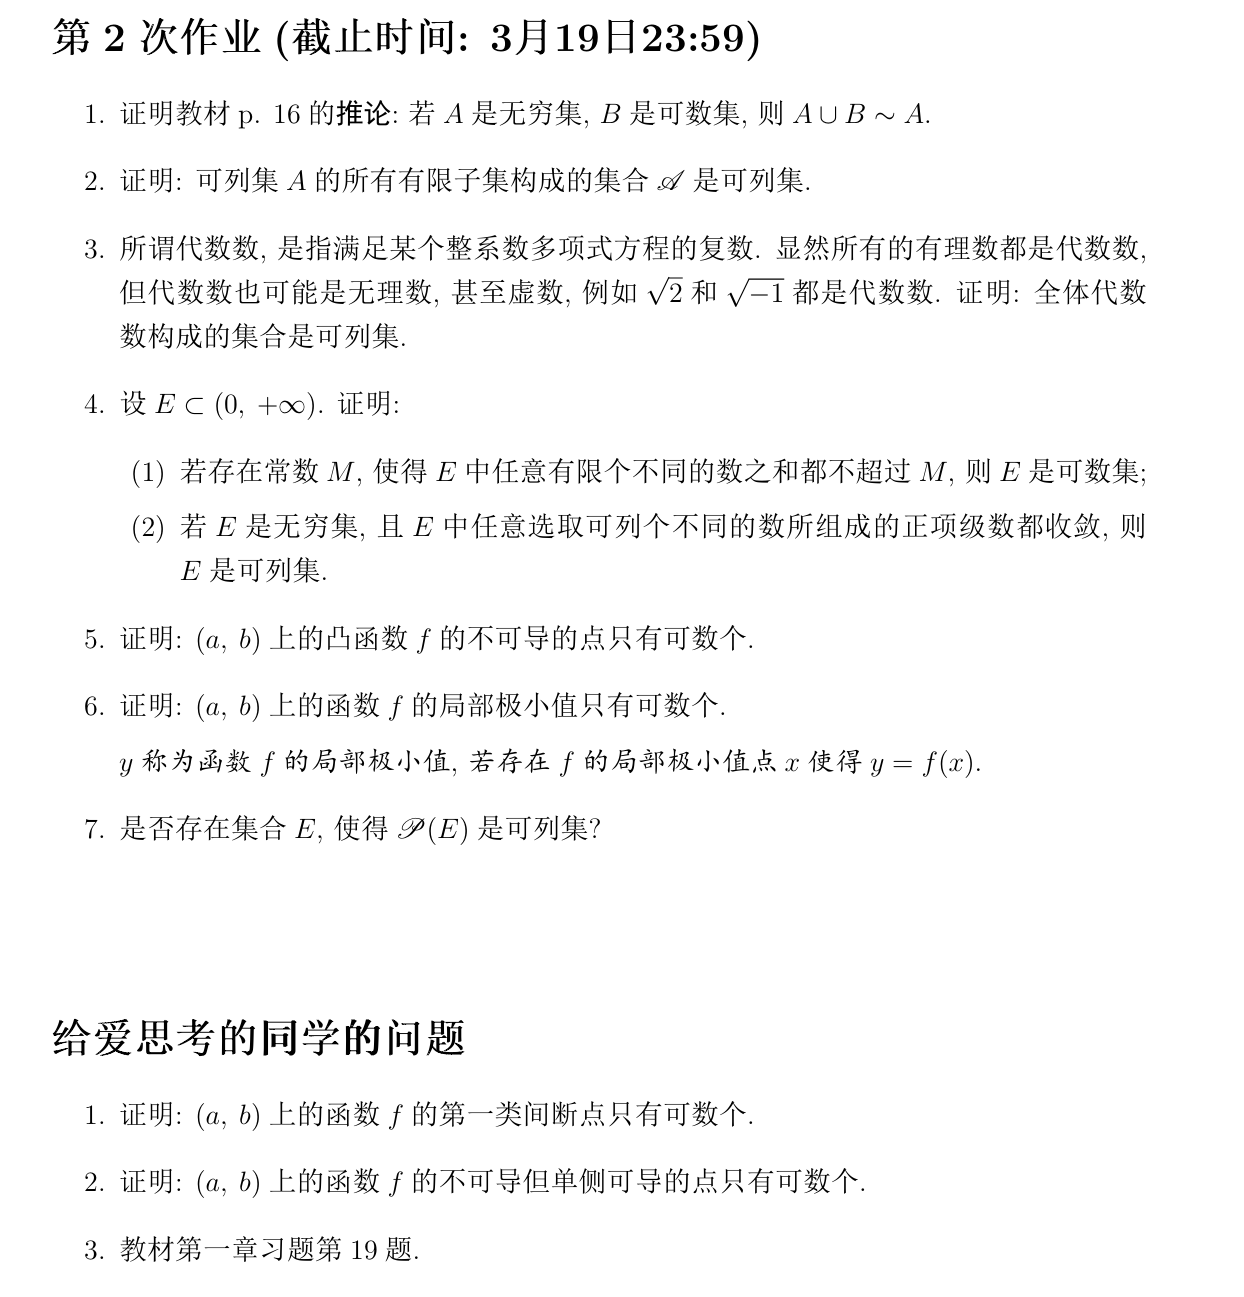
\includegraphics[width=\textwidth]{hw2-20250312.png}
% \caption{}
\label{}
\end{figure}

\begin{exercise}
若 $A$ 是无穷集,$B$ 是可数集,则 $A \cup B \sim A$ .
\end{exercise}
只需要建立一个一一映射,用来说明 $A\cup B$ 和 $A$ 的元素个数一样多。

\begin{theorem}
\begin{figure}[H]
\centering
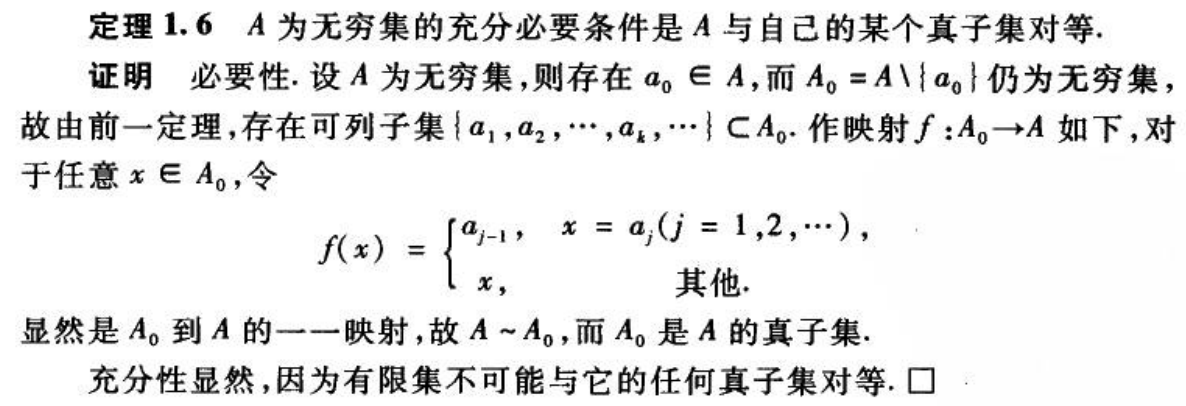
\includegraphics[width=\textwidth]{2-hw2-20250312.png}
% \caption{}
\label{}
\end{figure}\label{a6b345}
\end{theorem}

不妨设 $A\cap B=\varnothing$. 由于 $B$ 可数,不妨设为 $\{ b_1,b_2,\dots,b_n,\dots \}$,由于 $A$ 是无穷集,根据 \cref{a6b345} 我们知道 $A\sim A_0$,其中 $A_0=A\setminus \{ a_1,a_2,\dots,a_n,\dots \}$,$\{ a_1,a_2,\dots \}\subset A$ 是一个可数集。那么我们构造映射如下
\[
f:A\cup B\to A_0\qquad x\mapsto\begin{cases}
a_{2j-1} & x=b_j \\
a_{2j} & x=a_j \\
x & otherwise
\end{cases}
\]
显然 $f(A\cup B)=A_0$,$x, y\in A\cup B,x\neq y\Rightarrow f(x)\neq f(y)$. 因此 $f$ 是一一映射,故 $A\cup B\sim A_0\sim A$.

\begin{exercise}
证明:可列集 $A$ 的所有有限子集构成的集合 $\mathscr{A}$ 是可列集.
\end{exercise}
不妨设 $A=\{ a_1,a_2,\dots,a_n,\dots \}$,构造一个嵌入映射
\[
f:\mathscr{A}\to \mathbb{Q}\qquad \{ a_i \}_{i\in I}\mapsto \sum_{i\in I}^{} 2^{-i}
\]
其中 $I\subset \mathbb{N}$ 有限,显然 $f$ 是一个单射,因此 $f:\mathscr{A\to}f(\mathscr{A})$ 是一个一一映射,由于 $f(\mathscr{A})\subset \mathbb{Q}$,所以 $f(\mathscr{A})$ 至多可数,故 $\mathscr{A}$ 至多可数。由于 $\{ a_i \}\in \mathscr{A},\forall i$,所以 $\mathscr{A}$ 不可能有限,因此 $\mathscr{A}$ 可数。

\begin{exercise}
所谓代数数,是指满足某个整系数多项式方程的复数.显然所有的有理数都是代数数,但代数数也可能是无理数,甚至虚数,例如 $\sqrt{2}$ 和 $\sqrt{-1}$ 都是代数数。证明:全体代数数构成的集合是可列集.
\end{exercise}
设全体代数数构成的集合为 $\mathscr{A}$,全体 $n$ 次整系数多项式构成的集合为 $P_n$,全体满足 $n$ 次整系数多项式方程的代数数构成的集合为 $\mathscr{A}_n$,我们构造如下的映射
\[
f_n:P_n\to \mathscr{A}_n\qquad \sum_{k=0}^{n} a_kx^{k}=a_n\prod_{k=1}^{n} (x-x_k)\mapsto(x_1,x_2,\dots ,x_n)
\]
显然 $\mathscr{A}=\bigcup_{n=1}^{\infty}f_n(P_n)$,由于可数集的可数并也是可数集,故只需要证明 $f_n(P_n)$ 都是至多可数集即可。由代数数的定义可知,$f_n$ 是一个满射,由于 $P_n\sim \mathbb{Z}^{n+1}$ 可数,所以 $\mathscr{A}_n=f_n(P_n)$ 至多可数。得证!

\begin{exercise}
设 $E \subset(0,+\infty)$ .证明:
(1)若存在常数 $M$ ,使得 $E$ 中任意有限个不同的数之和都不超过 $M$ ,则 $E$ 是可数集;
(2)若 $E$ 是无穷集,且 $E$ 中任意选取可列个不同的数所组成的正项级数都收敛,则 $E$ 是可列集.
\end{exercise}
(1) 显然 $\sup E\leq M<\infty$,不妨设 $M=1$,否则用 $\left\{  \frac{x}{M}:x\in E  \right\}$ 代替 $E$。由于 $E$ 中任意有限个不同的数之和不超过 $M=1$,那么 $\#(E\cap(1/n,1])\leq n$,又因为
\[
E=E\cap(0,1]=E\cap\left( \bigcup_{n=1}^{\infty} (1/n,1] \right)=\bigcup_{n=1}^{\infty} (E\cap(1/n,1])
\]
是一列至多可数集的可数并,故 $E$ 至多可数。
(2) 考虑
\[
E=\left\{  \{ a_1,a_2,\dots \}\subset E:\sum_{n=1}^{\infty} a_n<\infty  \right\}=\bigcup_{m=1}^{\infty} \left\{  \{ a_1,a_2,\dots \}\subset E:\sum_{n=1}^{\infty} a_n<m  \right\}\eqqcolon \bigcup_{m=1}^{\infty} A_m
\]
由 (1) 可知:存在常数 $m$ 使得 $A_m$ 中任意有限个不同的数之和都不超过 $m$,于是 $A_m$ 是至多可数集。由于至多可数集的可数并可数。所以 $E=\bigcup_{n=1}^{\infty}A_n$ 可数。

\begin{exercise}
证明:$(a, b)$ 上的凸函数 $f$ 的不可导的点只有可数个.
\end{exercise}
根据凸函数的定义,对于任意 $(x,y)\subset(a,b)$,对于任意 $\lambda\in(0,1)$,我们有
\[
\lambda f(x)+(1-\lambda)f(y)\leq f(\lambda x+(1-\lambda)y)
\]
任意给定 $x\in(a,b)$,考虑函数
\[
g(y)=\frac{f(y)-f(x)}{y-x}\qquad y\in(a,b)\setminus \{ x \}
\]
显然 $g(y)$ 在 $(a,x)$ 和 $(x,b)$ 上分别单调递减,显然 $g(y)$ 在 $(a,x)$ 上单调递减且有下界 $\frac{f\left( \frac{x+b}{2} \right)-f(x)}{\frac{x+b}{2}-x}$,于是 $\lim_{ y \to x^{-} }g(y)=f'(x-)$ 存在,由于 $g(y)$ 在 $(x,b)$ 上单调递减且有上界 $\frac{f\left( \frac{a+x}{2} \right)-f(x)}{\frac{a+x}{2}-x}$,于是 $\lim_{ y \to x^{+} }f(y)=f'(x+)$ 存在。定义集合
\[
C=\{ x\in(a,b):f'(x-)\neq f'(x+) \}
\]
由于 $f$ 的凸性,我们知道 $f'(x-)\leq f'(x+)$。因此,对于 $x\in C$,考虑区间 $(f'(x-),f'(x+))$,由于 $\mathbb{Q}$ 在 $\mathbb{R}$ 中稠密,$\mathbb{Q}\cap(f'(x-),f'(x+))\neq \varnothing$,任取 $\mathbb{Q}\cap(f'(x-),f'(x+))$ 的一个代表元 $r_{x}$,我们得到如下的嵌入映射
\[
F:C\to \mathbb{Q}\qquad x\mapsto r_{x}
\]
显然这是一个单射,那么 $C\sim F(C)\subset \mathbb{Q}$,于是 $C$ 至多可数。

\begin{exercise}
证明:$(a, b)$ 上的函数 $f$ 的局部极小值只有可数个.
\end{exercise}
考虑集合
\[
C=\{ x\in(a,b):x\text{是}f \text{的局部极小值点} \}\quad D=\{ y=f(x):x\in C \}
\]
由局部极小值的定义可知,$D$ 是 $f$ 的全部局部极小值构成的集合,显然 $\#D \leq\# C$. 只需证明集合 $C$ 至多可数即可。
对于任意的 $x\in C$,将 $(a,x)$ 中离 $x$ 最近的极小值点记作 $x'$,将 $(x,b)$ 中离 $x$ 最近的极小值点记作 $x''$. 由于 $x$ 是一个局部极小值点,所以存在 $x$ 的一个充分小的邻域 $U_{x}\subset(x',x'')$,使得 $f (y)\geq f (x),\forall y\in U_{x}$。让 $x$ 取遍 $C$ 中的所有元素,这样得到的所有 $U_{x}$ 两两无交。对于任意给定的 $x\in C$,由于 $\mathbb{Q}$ 在 $\mathbb{R}$ 中稠密,可以任取一个 $r_{x}\in \mathbb{Q}\cap U_{x}$ 作为代表元,构造如下嵌入映射
\[
F:C\to \mathbb{Q}\qquad x\mapsto r_{x}
\]
这显然是一个单射,于是 $C\sim F(C)\subset \mathbb{Q}$,于是 $C$ 至多可数。

\begin{exercise}
是否存在集合 $E$ ,使得 $\mathscr{P}(E)$ 是可列集?
\end{exercise}
$\mathscr{P}(E)$ 表示 $E$ 的幂集,这是一个 $\sigma$ 代数,若 $E$ 有限,那么显然 $\# \mathscr{P}(E)=2^{\lvert E \rvert}$ 有限。若 $E$ 无限,假设 $\mathcal{A=}\{ A_1,A_2,\dots,A_n,\dots \}$ 是 $E$ 的一个可数子集,不是一般性,我们不妨假设 $\mathcal{A}$ 中集合两两无交,否则令
\[
\overline{A}_{1}=A_1,\quad \overline{A}_{2}=A_2\setminus A_1,\dots,\overline{A}_n=A_n\setminus\left( \bigcup_{k=1}^{n-1} A_k \right),\dots
\]
由于 $\mathscr{P}(E)$ 表示 $E$ 的幂集,必然有 $\mathscr{P}(\mathcal{A})\subset \mathscr{P}(E)$。断言 $\mathscr{P}(A)$ 不可数,我们现在考虑 $\mathscr{P}(A)$ 的任意一列子集 $S_1,S_2,\dots$,构造一个新的子集 $S$:若 $A_n\in S_n$,则 $A_n \not\in S_n$,否则 $A_n\in S_n$。于是 $S\not\in \{ S_1,S_2,\dots. \}$,但 $S\in \mathscr{P}(A)$. 这意味着 $\mathscr{P}(A)$ 的任意一个可数子集都是真子集,若 $\mathscr{P}(A)$ 可数,那么 $\mathscr{P}(A)$ 便是它自身的真子集,这与真子集的定义矛盾!故 $\mathscr{P}(A)$ 不可数,因此 $\mathscr{P}(E)$ 包含一个不可数集,故也不可数。
综上,不存在集合 $E$ 使得 $\mathscr{P}(E)$ 可列。

\begin{exercise}
证明:$(a, b)$ 上的函数 $f$ 的第一类间断点只有可数个.
\end{exercise}
记
\[
C=\{ x\in(a,b):x\text{是}f\text{的第一类间断点} \}
\]
固定 $x\in C$,记 $x'$ 是 $x$ 左侧最近的第一类间断点,$x''$ 是 $x$ 右侧最近的第一类间断点。$x'<x<x''$,根据有理数的稠密性,任取 $r_{x}\in\left( \frac{x'+x}{2},\frac{x+x''}{2} \right)$,构造如下映射
\[
F:C\to \mathbb{Q}\qquad x\mapsto r_{x}
\]
这显然是一个单射,于是 $C\sim F(C)\subset \mathbb{Q}$ 至多可数。

\begin{exercise}
证明:$(a, b)$ 上的函数 $f$ 的不可导但单侧可导的点只有可数个.
\end{exercise}
记
\[
C=\{ x\in(a,b):f\text{在}x\text{处不可导但单侧可导} \}=\{ x\in(a,b):f'(x-)\neq f'(x+) \}
\]
固定 $x\in C$,记 $x'$ 是 $x$ 左侧最近的不可导但单侧可导的点,$x''$ 是 $x$ 右侧最近的不可导但单侧可导的点。$x'<x<x''$,根据有理数的稠密性,任取 $r_{x}\in\left( \frac{x'+x}{2},\frac{x+x''}{2} \right)$,构造如下映射
\[
F:C\to \mathbb{Q}\qquad x\mapsto r_{x}
\]
这显然是一个单射,于是 $C\sim F(C)\subset \mathbb{Q}$ 至多可数。

\begin{exercise}
教材第一章习题第 19 题.
19.设 $E \subset \mathbf{R}^2$ 且为可数集,试构造 $E$ 的一个分解 $E=A \cup B$ ,使得平行于 $x$ 轴的直线与 $A$ 的交点为可数个,平行于 $y$ 轴的直线与 $B$ 的交点为可数个.
\end{exercise}
这是显然的!
